\section{Tablas de Mediciones}

A continuación, se presentan las tablas estructuradas para el registro de los datos experimentales obtenidos durante la sesión de laboratorio. Estas tablas permiten confrontar las mediciones directas e indirectas con los valores nominales o de catálogo proporcionados por el fabricante, facilitando el análisis de las desviaciones y el comportamiento del contactor.

\begin{table}[H]
    \centering
    \caption{Parámetros eléctricos y de operación del contactor electromagnético.}
    \label{tab:mediciones}
    \begin{tabularx}{\textwidth}{| X | c | Y | Y | c |}
        \hline
        \textbf{Parámetro} & \textbf{Símbolo} & \textbf{Valor Medido/\allowbreak Experimental} & \textbf{Valor Nominal/\allowbreak Catálogo} & \textbf{Unidades} \\ \hline
        Resistencia de la bobina & $R_{\text{bobina}}$ & & & \\ \hline
        Corriente de llamada & $I_{\text{llamada}}$ & & & \\ \hline
        Corriente de mantenimiento & $I_{\text{mantenimiento}}$ & & & \\ \hline
        Tensión de mantenimiento & $V_{\text{mantenimiento}}$ & & & \\ \hline
        Tensión mínima de operación / cierre & $V_{\text{operación}}$ & & & \\ \hline
    \end{tabularx}
\end{table}

En la figura~\ref{fig:caracteristicas_schneider} se presenta un extracto de catálogo de características de contactores comerciales Schneider Electric, sirviendo como ejemplo de los datos de placa/catálogo a registrar.

\begin{figure}[H]
    \centering
    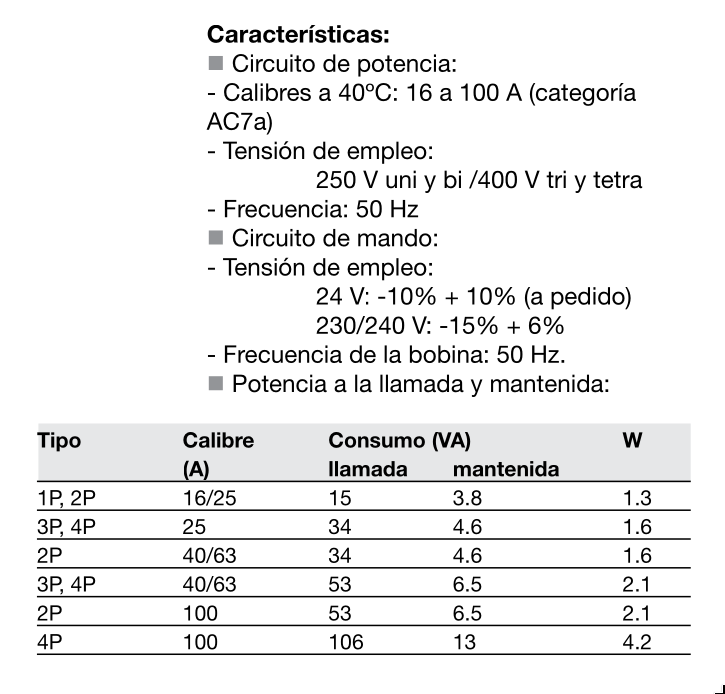
\includegraphics[width=0.8\textwidth]{figures/caracteristicas-contactor-ct.png}
    \caption{Especificaciones técnicas típicas de catálogo para contactores comerciales (Schneider Electric).}
    \label{fig:caracteristicas_schneider}
\end{figure}

